\section{Introduction}
YOLO (You Only Look Once) is a state-of-art algorithm devoted to object detection, as the name implies it can predict objects just by looking once at the image in a clever way. YOLO makes the prediction by classifying the object and locating it in the image. It uses deep learning and CNN techniques to detect objects, and distinguishes itself from its competitors because, as its name indicates, it requires to see the image only once, allowing it to be the fastest of all although it sacrifices a little accuracy. This speed allows users to easily detect objects in real time in videos (up to 30 FPS). In other words, YOLO takes as input value an image and passes through the neural network that looks like a CNN and returns a vector of bounding boxes and class prediction. To understand better how YOLO makes the prediction we will explain it with an example of an image as it can be seen in figure 3.1:
\newpage

\begin{figure}[h]
    \centering
    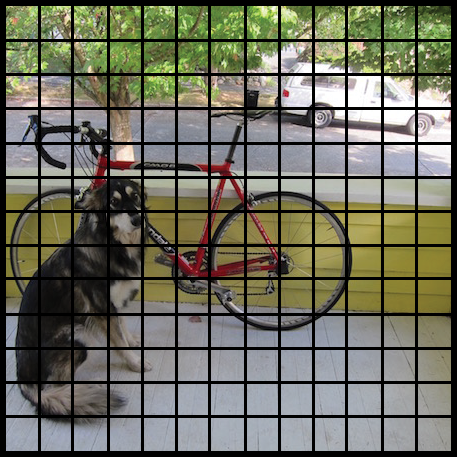
\includegraphics[max width=\textwidth]{images/ours/yolo-grid.png}
   \caption[Initial YOLO bounding boxes]{ YOLO divides up the image into a grid of 13 by 13 cells: Each of these cells is responsible for predicting 5 bounding boxes. A bounding box describes the rectangle that encloses an object. }
    \label{fig:yolo-grid}
\end{figure}



\section{YOLO in brief}
To perform de detection YOLO first divides the image into an S x S grid of cells, in Figure Figure 3.1 we can see that the image is divided into a 13 x 13 grid of cells. In each of the cells it predicts N possible bounding boxes and calculates the level of certainty (probability) of each of them (shown in Figure 13), that is, S x S x N different bounding boxes are calculated in the image, the vast majority of them with a very low level of certainty. The score of each BB does not classify what type of object is or it does not know what object is fitting the bounding box, it just gives a confidence value or a probability value of how good the BB is surrounding an object in each cell. In case of Figure Figure 3.1 for each grid cells 5 bounding boxes are predicted and are graphically shown in Figure 3.2 where the higher the probability is the fatter the box is. Each cell makes N bounding box predictions and M class probabilities. 

\begin{figure}[h]
    \centering
    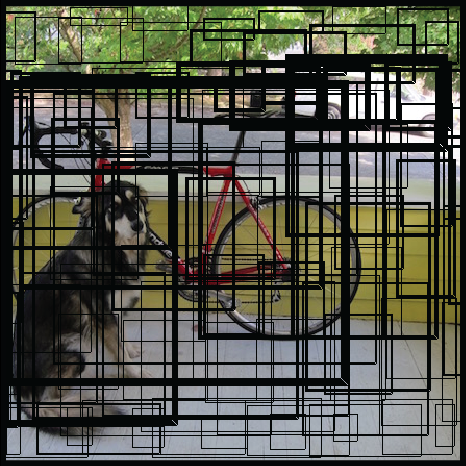
\includegraphics[max width=\textwidth]{images/ours/yolo-grid-2.png}
   \caption[The predicted bounding boxes]{ The predicted bounding boxes may look something like this, the higher the confidence score, the fatter the box is drawn. }
    \label{fig:yolo-grid-2}
\end{figure}

The bounding box prediction is formed by 5 components: x, y, width,
height, confidence score.

\begin{itemize}
\item The (x, y) components are like a mathematical graph coordinates that
refer to the centre of the box, relative to the grid cell location. If the
centre of the bounding box does not fall inside the grid cell this means
that the grid cell is not responsible of the object that has predicted the
bounding box. This happens because each object that appears in the image is related to a single grid cell that is responsible for predicting the
object. (x, y) are normalized between 0 and 1.

\item (Width, height) represent the dimension of the box that contains an object,
they are also normalized to values from 0 to 1 and they are fundamental
to locate the object in the image.

\item Confidence score is a real value that represents the assurance the algorithm has that the box contains an object of any class. The method how
the confidence is calculated will be explained later.

\end{itemize}


\section{The Predictions Vector}
The first step to understanding YOLO is how it encodes its output. The input image is divided into an S x S grid of cells. For each object that is present on the image, one grid cell is said to be “responsible” for predicting it. That is the cell where the center of the object falls into. 

Each grid cell predicts B bounding boxes as well as C class probabilities. The bounding box prediction has 5 components: (x, y, w, h, confidence). The (x, y) coordinates represent the center of the box, relative to the grid cell location (remember that, if the center of the box does not fall inside the grid cell, then this cell is not responsible for it). These coordinates are normalized to fall between 0 and 1. The (w, h) box dimensions are also normalized to [0, 1], relative to the image size.

\begin{figure}[h]
    \centering
    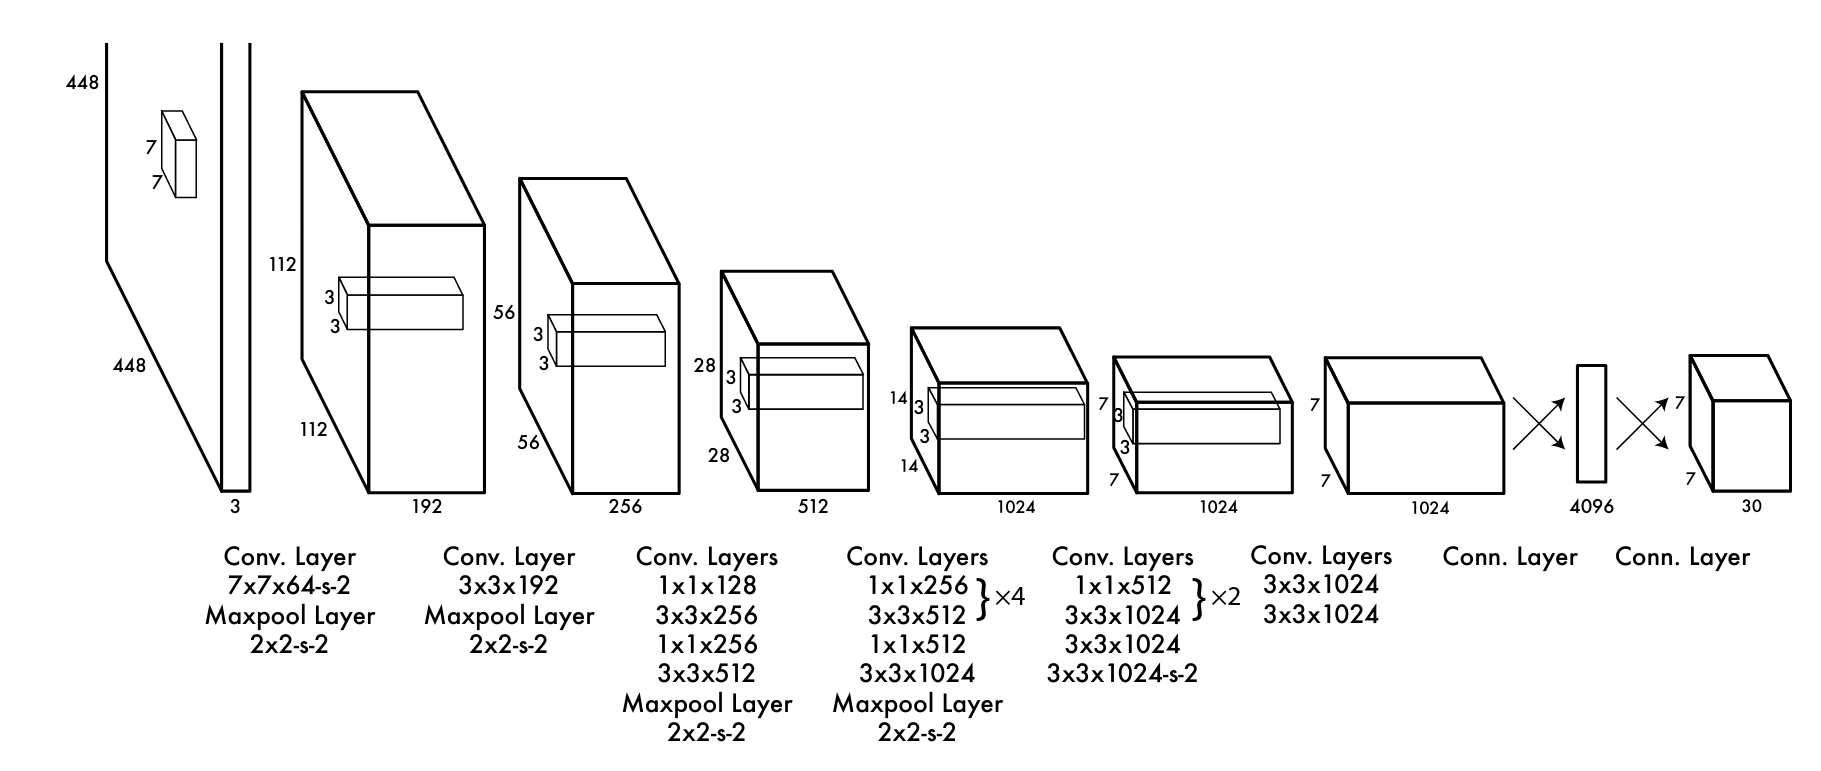
\includegraphics[max width=\textwidth]{images/ours/layers.png}
   \caption[The YOLOv5 Architecture]{ The Architecture. Our detection network has 24 convolutional layers followed
by 2 fully connected layers. Alternating 1 × 1 convolutional layers reduce the
features space from preceding layers. We pretrain the convolutional layers on the
ImageNet classification task at half the resolution (224 × 224 input image) and
then double the resolution for detection.
 }
    \label{fig:yolo-layers}
\end{figure}

\section{The Network}
The Architecture. Our detection network has 24 convolutional layers followed
by 2 fully connected layers. Alternating 1 ×1 convolutional layers reduce the
features space from preceding layers. We pretrain the convolutional layers on
the ImageNet classification task at half the resolution (224 ×224 input image)
and then double the resolution for detection.


The network structure looks like a normal CNN, with convolutions and max pooling layers, followed by 2 fully connected layers in the end: Note that the architecture was crafted for use in the Pascal VOC dataset, where the authors used S= 7, B = 2 and C = 20. This explains why the final feature maps are 7×7, and also explains the size of the output (7x7x (2×5+20)). Use of this network with a different grid size or different number of classes might require tuning of the layer dimensions. The authors mention that there is a fast version of YOLO, with fewer convolutions layers. We can see that in Table 3.1


\begin{table}[hbt!]
  \centering
  \caption[YOLO Network Structure]{YOLO Network Structure}
  \label{tab:orig-yolo-network}
  {\renewcommand{\arraystretch}{1.5}
    \begin{tabular}{p{0.33\textwidth} p{0.33\textwidth} p{0.33\textwidth}}
      \toprule
      Name       &        Filters         & Output Dimension  \\
      \hline
      Conv 1     & 7 x 7 x 64, stride=2   & 224 x 224 x 64    \\
      Max Pool 1 & 2 x 2, stride=2        & 112 x 112 x 64    \\
      Conv 2     & 3 x 3 x 192            & 112 x 112 x 192   \\
      Max Pool 2 & 2 x 2, stride=2        & 56 x 56 x 192     \\
      Conv 3     & 1 x 1 x 128            & 56 x 56 x 128     \\
      Conv 4     & 3 x 3 x 256            & 56 x 56 x 256     \\
      Conv 5     & 1 x 1 x 256            & 56 x 56 x 256     \\
      Conv 6     & 1 x 1 x 512            & 56 x 56 x 512     \\
      Max Pool 3 & 2 x 2, stride=2        & 28 x 28 x 512     \\
      Conv 7     & 1 x 1 x 256            & 28 x 28 x 256     \\
      Conv 8     & 3 x 3 x 512            & 28 x 28 x 512     \\
      Conv 9     & 1 x 1 x 256            & 28 x 28 x 256     \\
      Conv 10    & 3 x 3 x 512            & 28 x 28 x 512     \\
      Conv 11    & 1 x 1 x 256            & 28 x 28 x 256     \\
      Conv 12    & 3 x 3 x 512            & 28 x 28 x 512     \\
      Conv 13    & 1 x 1 x 256            & 28 x 28 x 256     \\
      Conv 14    & 3 x 3 x 512            & 28 x 28 x 512     \\
      Conv 15    & 1 x 1 x 512            & 28 x 28 x 512     \\
      Conv 16    & 3 x 3 x 1024           & 28 x 28 x 1024    \\
      Max Pool 4 & 2 x 2, stride=2        & 14 x 14 x 1024    \\
      Conv 17    & 1 x 1 x 512            & 14 x 14 x 512     \\
      Conv 18    & 3 x 3 x 1024           & 14 x 14 x 1024    \\
      Conv 19    & 1 x 1 x 512            & 14 x 14 x 512     \\
      Conv 20    & 3 x 3 x 1024           & 14 x 14 x 1024    \\
      Conv 21    & 3 x 3 x 1024           & 14 x 14 x 1024    \\
      Conv 22    & 3 x 3 x 1024, stride=2 & 7 x 7 x 1024      \\
      Conv 23    & 3 x 3 x 1024           & 7 x 7 x 1024      \\
      Conv 24    & 3 x 3 x 1024           & 7 x 7 x 1024      \\
      FC 1       & -                      & 4096              \\
      FC 2       & -                      & 7 x 7 x 30 (1470) \\
\bottomrule
    \end{tabular}
  }
\end{table}

Note that the architecture was crafted for use in the Pascal VOC dataset, where the authors used $S=7$, $B=2$ and $C=20$. This explains why the final feature maps are $7 \times 7$, and also explains the size of the output $(7x7x(2 \times 5+20))$. Use of this network with a different grid size or different number of classes might require tuning of the layer dimensions. The authors mention that there is a fast version of YOLO, with fewer convolutional layers. The table~\ref{tab:orig-yolo-network}, however, display the full version. The sequences of 1x1 reduction layers and 3x3 convolutional layers were inspired by the GoogLeNet (Inception) model. The final layer uses a linear activation function. All other layers use a leaky RELU $(\phi(x) = x, if x>0; 0.1x \ otherwise)$.

\section{The Loss Function}
The loss function start like this:
\begin{equation}
  \lambda_{coord} \sum_{i=0}^{S^2}\sum_{j=0}^B \mathbbm{1}_{ij}^{obj}[(x_i-\hat{x}_i)^2 + (y_i-\hat{y}_i)^2 ]
\label{yolo-loss-func}
\end{equation}

This equation computes the loss related to the predicted bounding box position $(x,y)$. Don’t worry about $\lambda$ for now, just consider it a given constant. The function computes a sum over each bounding box predictor $(j = 0..B)$ of each grid cell $(i = 0 .. S^2)$. $\mathbbm{1} obj$ is defined as follows:

\begin{itemize}
  \item 1, If an object is present in grid cell i and the jth bounding box predictor is “responsible” for that prediction
  \item 0, otherwise
\end{itemize}

But how do we know which predictor is responsible for the object? Quoting the original paper:
\begin{quote}
YOLO predicts multiple bounding boxes per grid cell. At training time we only want one bounding box predictor to be responsible for each object. We assign one predictor to be “responsible” for predicting an object based on which prediction has the highest current IOU with the ground truth.
\end{quote}

The other terms in the equation should be easy to understand: $(x, y)$ are the predicted bounding box position and $(\hat{x}, \hat{y})$ hat are the actual position from the training data.

Let’s move on to the second part:
\begin{equation}
  \lambda_{coord} \sum_{i=0}^{S^2}\sum_{j=0}^B \mathbbm{1}_{ij}^{obj}[(\sqrt{w_i}-\sqrt{\hat{w}_i})^2 +(\sqrt{h_i}-\sqrt{\hat{h}_i})^2 ]
\label{yolo-loss-func-2}
\end{equation}


This is the loss related to the predicted box width / height. The equation looks similar to the first one, except for the square root. Quoting the paper again:

\begin{quote}
Our error metric should reflect that small deviations in large boxes matter less than in small boxes. To partially address this we predict the square root of the bounding box width and height instead of the width and height directly.
  \end{quote}

    

Moving on to the third part:
\begin{equation}
  \sum_{i=0}^{S^2}\sum_{j=0}^B \mathbbm{1}_{ij}^{obj}(C_i - \hat{C}_i)^2 + \lambda_{noobj}\sum_{i=0}^{S^2}\sum_{j=0}^B \mathbbm{1}_{ij}^{noobj}(C_i - \hat{C}_i)^2
\label{yolo-loss-func-3}
\end{equation}


Here we compute the loss associated with the confidence score for each bounding box predictor. $C$ is the confidence score and $\hat{C}$ is the intersection over union of the predicted bounding box with the ground truth. $\mathbbm{1} obj$ is equal to one when there is an object in the cell, and 0 otherwise. $\mathbbm{1} noobj$  is the opposite.

The $\lambda $ parameters that appear here and also in the first part are used to differently weight parts of the loss functions. This is necessary to increase model stability. The highest penalty is for coordinate predictions $(\lambda coord = 5)$ and the lowest for confidence predictions when no object is present $(\lambda noobj = 0.5)$.

The last part of the loss function is the classification loss:
\begin{equation}
  \sum_{i=0}^{S^2} \mathbbm{1}_{i}^{obj}\sum_{c \in classes}(p_i(c) - \hat{p}_i(c))^2
\label{yolo-loss-func-4}
\end{equation}

It looks similar to a normal sum-squared error for classification, except for the $\mathbbm{1} obj$ term. This term is used because so we don’t penalize classification error when no object is present on the cell (hence the conditional class probability discussed earlier).

Note that the loss function only penalizes classification error if an object is present in that grid cell (hence the con-ditional class probability discussed earlier). It also only pe-nalizes bounding box coordinate error if that predictor is “responsible” for the ground truth box (i.e. has the highest IOU of any predictor in that grid cell). \cite{redmon2016look}

